\hspace{4em}MOPy, a learning tool designed to learn and practice various orbital mechanics concepts. It is designed in a way such that it can be a user-friendly tool that can be operated with ease even by the user who has very limited knowledge about the concepts of orbital mechanics. It provides users to learn about a particular concept with a brief explanation so the user can gain the theoretical knowledge required through visualizations. The sophisticated 3D environment benefits the user to visualize the fundamental concepts easily. It assists the user to verify manually calculated data. It serves as advanced virtual calculator. MOPy is an open source software with GNU-GPL v3 license\cite{lic} which anyone can use or work with. It runs on windows platforms at present.
\begin{figure}[H]
\centering

\includegraphics[scale=0.24]{images/mopy.png}
\caption{MOPy} \label{mopy}
\end{figure}
\subsection{Features}
\begin{center}
\begin{table}[H]
{\rowcolors{2}{white}{gray!50}
\begin{tabular}{c|K{7.5cm}}
\hline 
Sl. No & \textbf{Section}\\ 
\hline 
1 & Calculation of Orbital Elements\\ 
\hline 
2 & 2D and 3D orbit \\ 
\hline 
3 & Various Parameters at any given point \\ 
\hline 
4 & 2D and 3D Orbits\\ 
\hline 
5 & Calculation of Julian Day \\ 
\hline 
5 & Euler Angles\\ 
\hline 
6 & Sphere Of Influence \\ 
\hline 
7 & Sensitivity Analysis \\ 
\hline 
8 & Position of one Spacecraft w.r.t Another\\ 
\hline 
9 & Calculation of State and Velocity Vector\\ 
\hline
10 & Orbital Transfer \\
\hline
\end{tabular}}
\caption{\label{tab: features}List of Features present in MOPy}
\end{table}
\end{center}
\subsection{Libraries Used}
\begin{enumerate}
\item \textbf{NumPy}:  This brings MATLAB like functionality of using Matrices and their operations to python. This enables us to do a lot of stuff without much hassle.
\item \textbf{SciPy} - This enables us to add many features involving more complex computing scenarios as it has features for scientific and technical computing. For example, it has different kinds of solvers for integration which we can use for solving acceleration vector equation to obtain the position vector for an orbit.
\item \textbf{Matplotlib} - This is a plotting tool that is a extension on NumPy that gives the functionality of plotting many different kinds of graph. This library is somewhat similar to the plotting feature of MATLAB.
\item \textbf{Panda3D} - This is a Game Engine based on C++ that takes in syntax from both C++ and Python. This provides real-time 3D visualizations and simulations based on the code.
\item \textbf{SQLite3} - The entire details of the planetary bodies like the orbital elements, planetary ephemeris and others are stored in a local database. SQLite is used as it enables the offline functionality.
\item \textbf{Qt Deisgner} - This enables MATLAB's App Designer like feature of dragging and dropping the UI elements and creating the GUI. This is based on Qt, a cross platform GUI toolkit developed by the Qt Company
\item \textbf{PyQt5 $\&$ PySide2} - These both are the python binding libraries of Qt.
\item \textbf{PyInstaller} - This library lets us convert our python code(.py) into executable file(.exe)
\end{enumerate}
\subsection{Market Research}
There are mainly two kinds of softwares.
\begin{enumerate}
\item Simulation Based programs like STK, FreeFlyer etc.,
\item Sandbox Based programs like Universe SandBox, Kerbal Space Program etc.,
\end{enumerate}
\hspace{4em}The simulation based programs are mainly used to simulate missions and solve problems based on the instance. Both the applications given in the example are used in the industry for all kinds of missions, ranging from very small scale missions that are performed by the students to complicated missions that are performed by NASA and ISRO.

The Sandbox based programs are the stuff that are run by the physics engine that are baked into it. They use a 3D visualization toolkit or engine which lets the user easily interact with the UI, and change the parameters directly from the environment.

In the analysis done by Morgan Stanley named \enquote{Investing in Space Exploration}, it is stated as - The revenue generated by the global space industry may increase to more than $\$$1 trillion by 2040. \cite{morgan}
\begin{figure}[H]
\centering
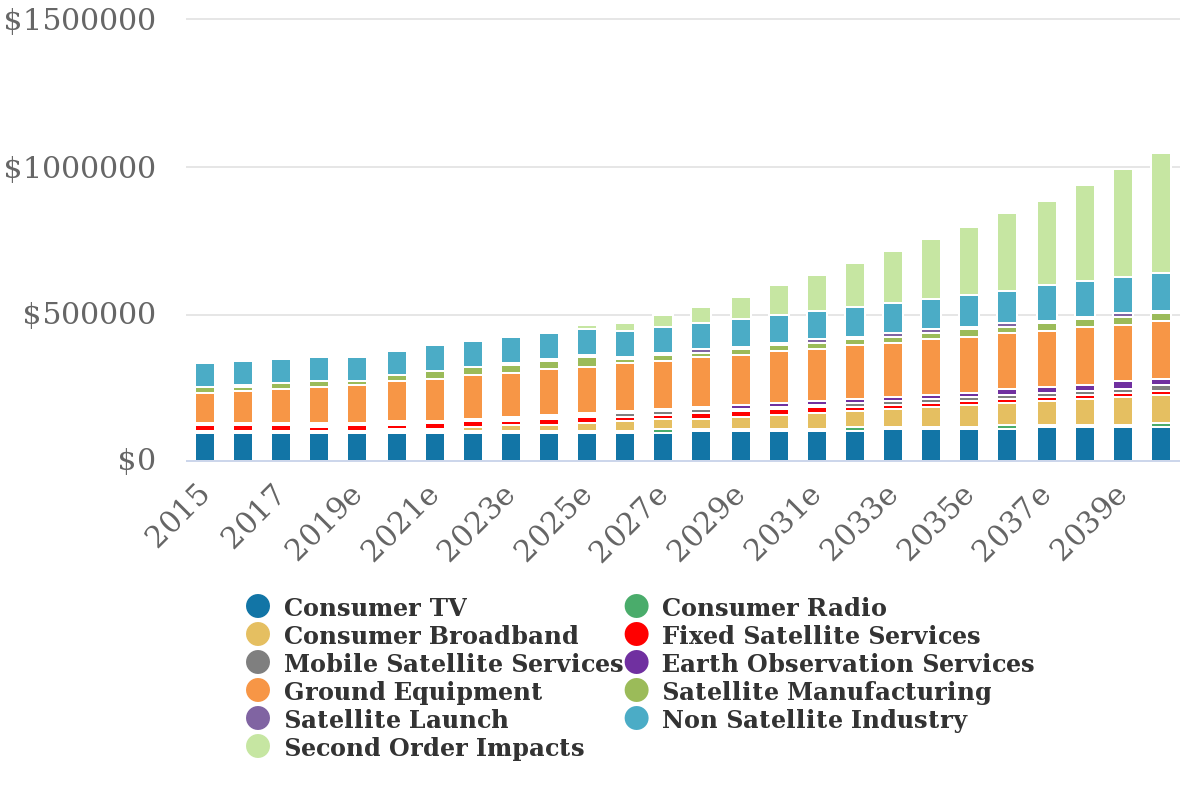
\includegraphics[scale=0.3]{images/morganstanley.png}
\caption{Global Market Trend according to Morgan Stanley.} \label{morgangraph}
\end{figure}
A report by Antrix and PwC, it is stated that the indian space sector can become a $\$$50 Billion industry, or about one per cent of India's projected $\$5$ Trillion economy, by 2024 from the current $\$7$ billion, according to a report by the Antrix and PwC.\cite{indiaspace}
\begin{figure}[H]
\centering
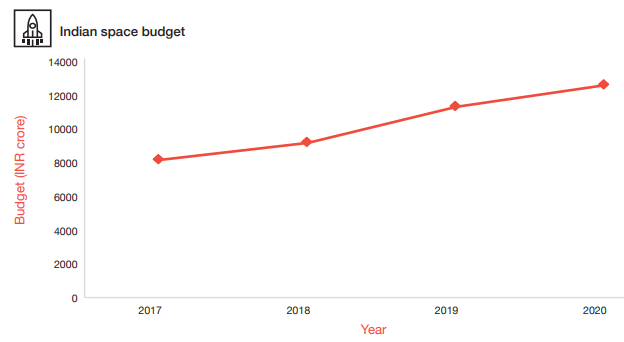
\includegraphics[scale=1.1]{images/pwc.png}
\caption{Indian Space Budget over the years.} \label{pwc}
\end{figure}
\subsection{Objective}
The development in the field of space technology is constantly increasing as shown in the aforementioned studies.
Such being the case, many students are showing interest to learn more and more about space technology and its related concepts. Considering all such possibilities, we have come up with an idea to develop a learning tool beneficial to learn more about Orbital Mechanics 
The main objectives of this project are as follows:
\begin{enumerate}
\item Design and develop a software to learn concepts and  solve Problems related orbital mechanics to understand the basics.
\item Provide a user friendly learning tool such that the user can operate even with the minimum knowledge about the concepts of orbital mechanics.
\item Help user to visualize the virtual view of the space mission.
\end{enumerate}
\subsection{Front End Development}
\subsubsection{Introduction}
Front-end development deals with the Graphical User-Interface aspect of the software. It is the key developmental process that defines how the user experiences the features we have developed. The interface between the user and the back end code is GUI. The inputs from the user is taken from the GUI. So the design must be intuitive and clear. There are many libraries that can be used to develop a GUI like PyQt, Pyside, Kivy, Tkinter, etc. In our case, we have opted for PyQt5, Pyside2 and designed GUI in Qt-Designer. Then linked the Back-End scripts through the Integrated Development Environment(IDE) by Microsoft i.e, Visual Studio Code.
\subsubsection{Home Page}
When the application opens the Home Page will load. In it, there is a Dropdown box containing all the features available, from which the user can choose which feature they want to use. When the user selects any of the features from the drop-down and clicks on the go button at the bottom, they are navigated to that screen where they can use the feature they selected. And then if they want to navigate back to the Home-Page they can click on the Home button provided at the top left corner of the screen. All the features are listed in the upper-mentioned table.
\begin{figure}[H]
\centering
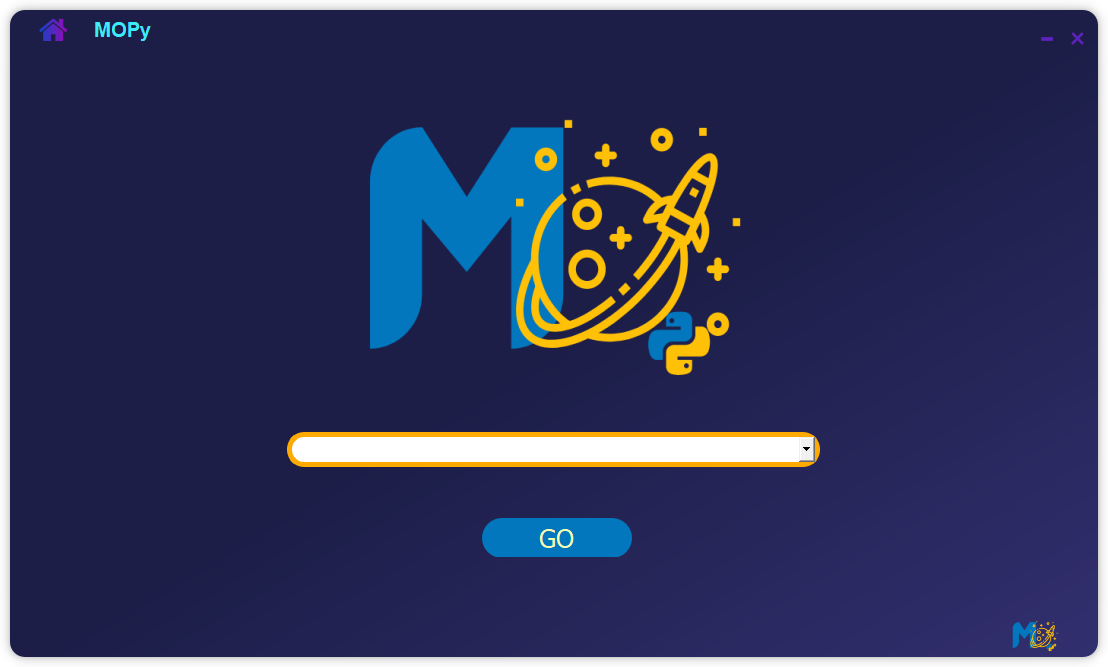
\includegraphics[scale=0.6]{images/homepage.png}
\caption{Home Page of MOPy} \label{home}
\end{figure}